\documentclass[]{article}

\title{Clustering e Classificazione}
\author{}
\usepackage{booktabs}
\usepackage{listings}
\usepackage{appendix}
\usepackage{graphicx}
\usepackage{multirow}

\lstset{
	frame=tb,
	language=SQL,
	aboveskip=3mm,
	belowskip=3mm,
	showstringspaces=false,
	columns=flexible,
	basicstyle={\small\ttfamily},
	numbers=left,
	stepnumber=1,
	breaklines=true,
	breakatwhitespace=true,
	tabsize=3
}

\begin{document}

\maketitle

\begin{abstract}

\end{abstract}

\section{Preprocessing e Database}
Per l'analisi del \textit{dataset} fornito basata sulle tecniche di clustering e di classificazione \`{e} stato predisposto un database MySQL per la gestione dei dati e per la creazione di alcune viste che facilitassero lo studio del dataset tramite tali tecniche. Il database utilizzato presenta le seguenti tabelle:
\begin{itemize}
	\item \textbf{students}: che contiene i dati principali legati agli studenti (\textit{student\_id}, \textit{cohort}, \textit{test\_grade}, \textit{hs\_diploma\_grade}, \textit{hs\_diploma\_title}). La tabella \`{e} stata popolata prelevando i dati dal file "\textit{anagrafica studenti}" fornito (\textit{students.csv}), selezionando tutti gli attributi presenti nel file.
	
	\item \textbf{courses}: che contiene i dati relativi ai corsi, prelevati dal file \textit{exams\_preproc.csv} ottenuto nella precedente fase di preprocessing per l'analisi dei pattern e selezionando dunque solo gli attributi \textit{course\_id}, \textit{cfu}, \textit{description}.
	 
	\item \textbf{exams}: che contiene i dati relativi agli esami sostenuti da ogni studente. Anche questa tabella \`{e} stata popolata prelevando i dati dal file ottenuto nella precedente fase di preprocessing e in particolare, selezionando gli attributi \textit{student\_id}, \textit{course\_id}, \textit{date}, \textit{grade}, \textit{semester}.
\end{itemize}

Tutte le tabelle sono state strutturate scegliendo le corrette chiave primarie e inserendo le chiavi esterne opportune. Di seguito viene riportato il codice SQL utilizzato per il caricamento dei dati nel database.

\lstinputlisting[caption={import\_data.sql}, language=SQL]{Code/import_data.sql}

\paragraph{}
Una volta strutturato e popolato le tabelle del database si \`{e} provveduto ad effettuare la fase di preprocessing, ovvero, la gestione dei dati mancanti, in parte eseguita direttamente nel database costruito, la costruzione delle viste necessarie alle analisi, lo studio della correlazione fra coppie di attributi e la normalizzazione di alcuni di essi per il corretto utilizzo degli algoritmi di clustering e di classificazione. 

Per gestire la mancanza di alcuni voti del test di ingresso nel dataset "anagrafica studenti" fornito, \`{e} stato deciso di integrare i voti mancanti con una media complessiva dei risultati del test di ingresso di tutti gli studenti, utilizzando una semplice query di UPDATE sulla tabella \textit{students}. Di seguito viene riportata la query SQL utilizzata.

\lstinputlisting[caption={preprocessing\_students\_table.sql}, language=SQL]{Code/preprocessing_students_table.sql}

\paragraph{}
Per quanto riguarda lo studio attraverso le tecniche di clustering si \`{e} deciso di fare due principali analisi:
\begin{enumerate}
	\item Sulla carriera e il percorso di ogni studente considerando dati come il voto ottenuto al test di ingresso, il voto di diploma e la media pesata del voto degli esami sostenuti, per cercare di raggruppare fra loro tutti gli studenti con carriere simili.
	
	\item Sull'andamento dei risultati di ogni esame degli studenti, per cercare di raggruppare fra loro gli studenti che hanno ottenuto delle votazioni simili rispetto agli esami.
\end{enumerate}
Al fine di eseguire le analisi sopra descritte sono state create rispettivamente le due seguenti viste in modo tale da raggruppare i dati necessari. Le viste sono state create in modo seguente.
\begin{itemize}
	\item \textbf{cluster\_career}: la quale contiene per ogni studente il voto al test di ingresso (\textit{test\_grade}), il voto di diploma (\textit{diploma\_grade}), la media pesata (sui \textit{cfu}) dei voti degli esami sostenuti e arrotondata (\textit{grade\_weighted\_avg}), il numero di esami sostenuti (\textit{exams\_taken}), il numero totale di cfu acquisiti (\textit{total\_cfu}) e un'ultima colonna con la differenza di anni tra la data dell'ultimo esame sostenuto e la corte dello studente (\textit{years}). Gli attributi precedentemente descritti sono stati ricavati tramite script SQL dagli attributi delle tabelle del database (\textit{Feature Creation}). Di seguito viene riportata una porzione della vista creata.
	
	\begin{center}
		\resizebox{\columnwidth}{!}{
		\begin{tabular}{lllllll}
			\hline
			student\_id & test\_grade & hs\_diploma\_grade & grade\_weighted\_avg & exams\_taken & total\_cfu & years \\ \hline
			A & 18 & 80 & 27.0 & 10 & 90 & 4 \\
			B & 13 & 67 & 23.0 & 10 & 96 & 4 \\
			C & 18 & 78 & 25.0 & 7 & 69 & 4 \\
			D & 14 & 66 & 23.0 & 7 & 66 & 2 \\
			E & 16 & 82 & 28.0 & 2 & 24 & 2 \\ \hline
		\end{tabular}
		}
	\end{center}

	\item \textbf{cluster\_exams}: la quale contiene per ogni studente i voti ottenuti ad ogni esame. Per questa vista, dato che molti studenti non hanno ancora sostenuto alcuni esami, abbiamo deciso di integrare i valori mancanti utilizzando la media dei voti dello studente. Tale modifica \`{e} stata fatta esportando la vista in un file \textit{.csv} (contenente dunque anche i dati mancanti) e modificando quest'ultimo con uno script python. Di seguito viene riportata una porzione della vista con i dati aggiornati.
	
	\begin{center}
		\resizebox{\columnwidth}{!}{
			\begin{tabular}{lllllll}
				\hline
				student\_id & B006800 & B006801 & B006802 & B006803 & B006804 & B006807 \\ \hline
				A & 29 & 30.0 & 25.0 & 25.9 & 30.0 & 24.0 \\
				B & 26 & 20.0 & 21.0 & 18.0 & 26.0 & 22.0 \\
				C & 28 & 24.7142 & 22.0 & 24.7142 & 26.0 & 24.7142 \\
				D & 20 & 28.0 & 22.0 & 23.1428 & 22.0 & 21.0 \\
				E & 28 & 27.0 & 27.5 & 27.5 & 27.5 & 27.5 \\ \hline
			\end{tabular}
		}
	\end{center}	
	
\end{itemize} 

Per la classificazione abbiamo invece deciso, come verr\`{a} spiegato meglio in seguito nella fase di postprocessing, di recuperare le classi dai risultati del clustering eseguito sulla prima vista \textit{cluster\_career}, essendo tali risultati i pi\`{u} significativi.\\
Per la creazione del database viene fornito in allegato alla relazione il codice SQL dell'intera creazione del database "database\_creation.sql" che ricrea completamente il database con i dati e le viste utilizzate.

\paragraph{}
Prima di applicare gli algoritmi di clustering e di classificazione sui dataset sono state fatte alcune analisi sui essi per comprendere meglio i dati a disposizione. \`{E} stata quindi calcolata la matrice di correlazione usando l'indice di \textit{Pearson} sui dati relativi alla vista \textit{cluster\_career} per capire quanto i vari attributi sono correlati tra loro.

\begin{figure}[h]
	\centering
	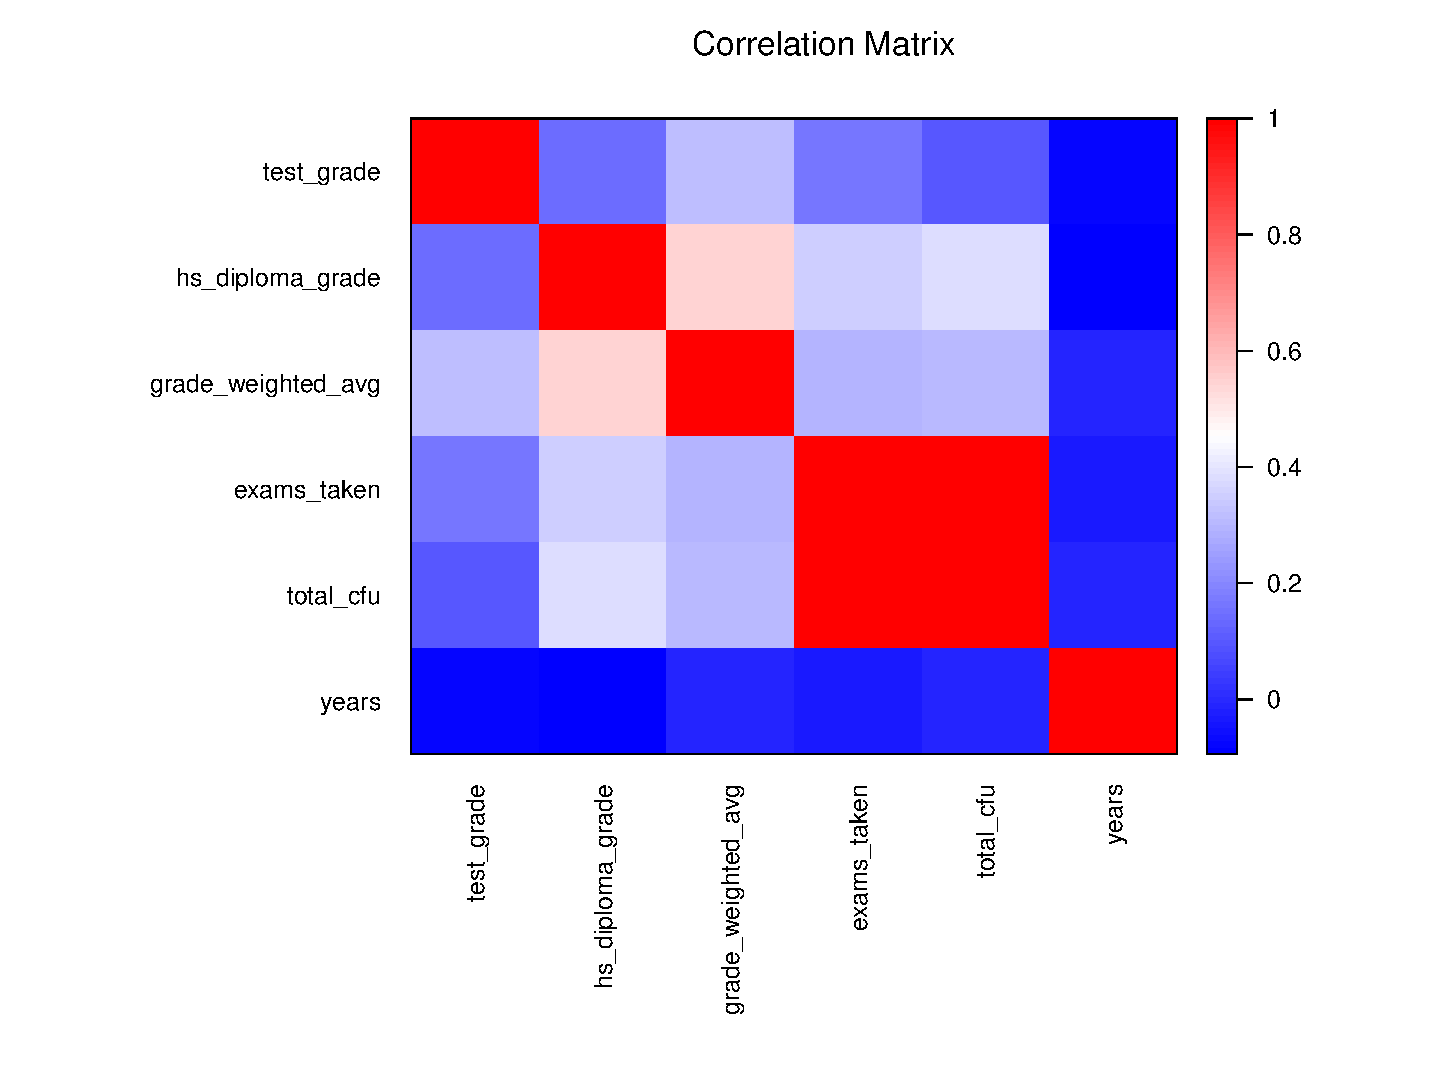
\includegraphics[scale=0.5]{Img/corr_matrix_career.pdf}
	\caption{Matrice di correlazione per \textit{cluster\_career}.
	\label{fig:1}}
\end{figure} 

\begin{center}
	\resizebox{\columnwidth}{!}{
		\begin{tabular}{l|llllll}
			& test\_grade & hs\_diploma\_grade & grade\_weighted\_avg & exams\_taken & total\_cfu & years \\ \hline
			test\_grade & 1 & 0.14486 & 0.32133 & 0.16350 & 0.098900 & -0.074509 \\
			hs\_diploma\_grade & 0.14486 & 1 & 0.54464 & 0.35031 & 0.381964 & -0.094038 \\
			grade\_weighted\_avg & 0.32133 & 0.54464 & 1 & 0.29749 & 0.303728 & -0.011494 \\
			exams\_taken & 0.16350 & 0.35031 & 0.29749 & 1 & 0.991599 & -0.038072 \\
			total\_cfu & 0.09890 & 0.38196 & 0.30372 & 0.99159 & 1 & -0.009638 \\
			years & -0.0745 & 0.009638 & -0.0114 & -0.0380 & -0.00963 & 1
		\end{tabular}
	}
\end{center}

Come si pu\`{o} vedere dalla heatmap in Figura \ref{fig:1} ed in modo specifico dalla matrice di correlazione, \`{e} presente un'interessante  discreta correlazione di circa $0,545$ tra la media pesata dei voti degli esami dello studente e il voto di diploma, lasciando dedurre che un buon risultato all'esame di maturit\`{a} comporti in genere una buona media degli esami universitari. C'\`{e} inoltre una forte correlazione tra gli esami sostenuti e il numero di CFU ottenuti dallo studente, tale risultato risulta tuttavia abbastanza intuitivo, in quanto al crescere degli esami sostenuti crescer\`{a} anche il numero di CFU acquisiti dallo studente e viceversa. Infine, la figura suggerisce come l'attributo \textit{year} risulti quasi totalmente non correlato al resto degli attributi, probabilmente per il fatto che per la maggior parte degli studenti di questo dataset dall'anno di immatricolazione fino all'ultimo esame sostenuto sono passati due anni. Il resto degli attributi non presentano valori di correlazione significativi.\\

\`{E} stata successivamente calcolata la matrice di correlazione usando Pearson sui dati relativi alla vista \textit{cluster\_exams} per scoprire anche su di essa gli attributi pi\`{u} correlati.

\begin{figure}[h]
	\centering
	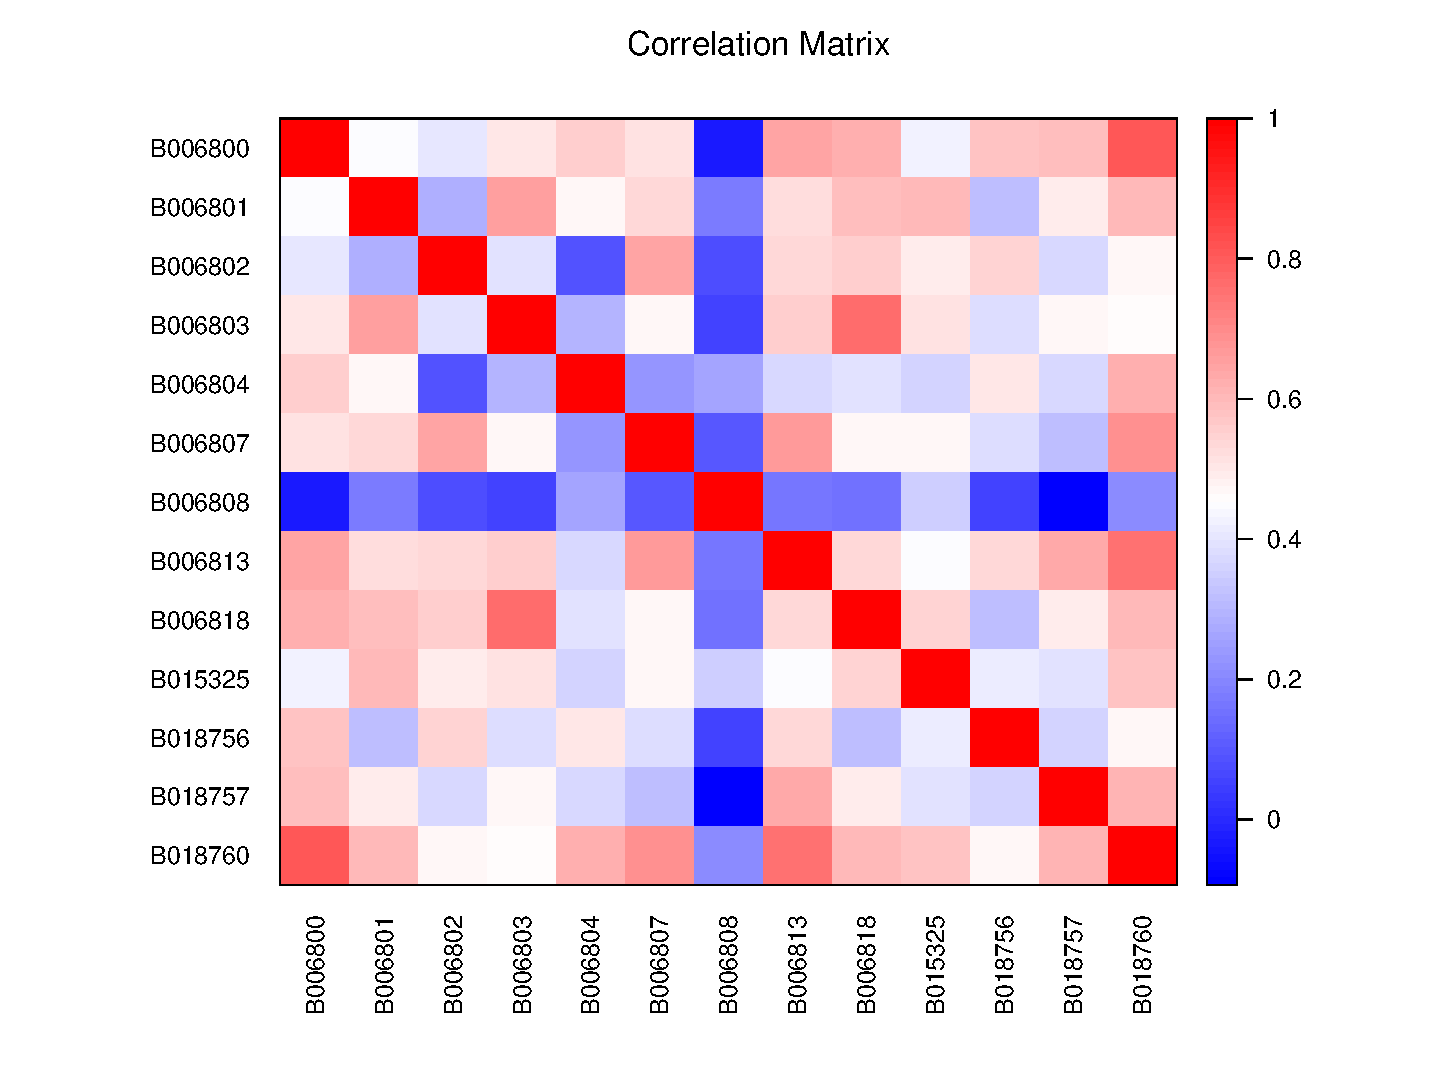
\includegraphics[scale=0.5]{Img/corr_matrix_exams.pdf}
	\caption{Matrice di correlazione per \textit{cluster\_exams}.
		\label{fig:2}}
\end{figure} 

Come si pu\`{o} vedere dalla heatmap di Figura \ref{fig:2}, abbiamo diversi esami che sembrano avere una correlazione nella distribuzione dei voti. Ad esempio esiste una forte correlazione dello $0.812$ tra l'esame di Algoritmi e Strutture Dati (B006800) e l'esame di Calcolo delle Probabilit\`{a} e Statistica (B018760), una correlazione dello $0.762$ tra Sistemi Operativi (B006818) e Matematica Discreta e Logica (B006803) ed una di $0.759$ tra BSDI (B006813) e CPS (B018760), le quali rappresentano le correlazioni pi\`{u} forti. La figura mostra inoltre come l'esame di Analisi II (B006808) risulti quasi totalmente incorrelato dal resto degli esami, in quanto la maggior parte degli studenti ha una votazione bassa oppure non hanno sostenuto l'esame. Queste correlazioni per\`{o} potrebbero essere imprecise dato l'alto numero di dati mancanti che mostrava il \textit{dataset} fornito, ovvero molti studenti che non hanno ancora sostenuto tutti gli esami.

\paragraph{}
Per applicare gli algoritmi di clustering al data set \`{e} stato utilizzato il software Weka, collegandolo direttamente al database MySQL per estrarre facilmente le viste sulle quali applicare gli algoritmi.

Prima di applicare gli algoritmi \`{e} stato per\`{o} eseguita un'ulteriore fase di preprocessing sui dati della vista \textit{cluster\_career} direttamente in Weka. Durante tale fase sono stati normalizzati tutti gli attributi della vista eccetto l'identificatore dello studente (\textit{student\_id}) in scala da 0 a 1 al fine di evitare problemi dovuti a scale di valori differenti per gli attributi. Per quanto riguarda invece la vista \textit{cluster\_exams} non \`{e} stata fatta nessuna normalizzazione sui dati in quanto ogni campo ha lo stesso range di valori, essendo tutti voti di esami da 18 a 31.\\

Tutte e due le viste predisposte per il clustering sono disponibili anche in due differenti file \textit{.csv}, rispettivamente nel file \textit{cluster\_career.csv} e \textit{cluster\_exams.csv} allegati a questa relazione per facilitare la riproduzione dei risultati nella fase di applicazione degli algoritmi di clustering.

\section{Clustering}
Come prima analisi si mostra quella relativa alla carriera dello studente usando i dati estrapolati dalla vista \textit{cluster\_career} resi disponibili nel file \textit{cluster\_career.csv}.\\

\begin{figure}[!]
	\centering
	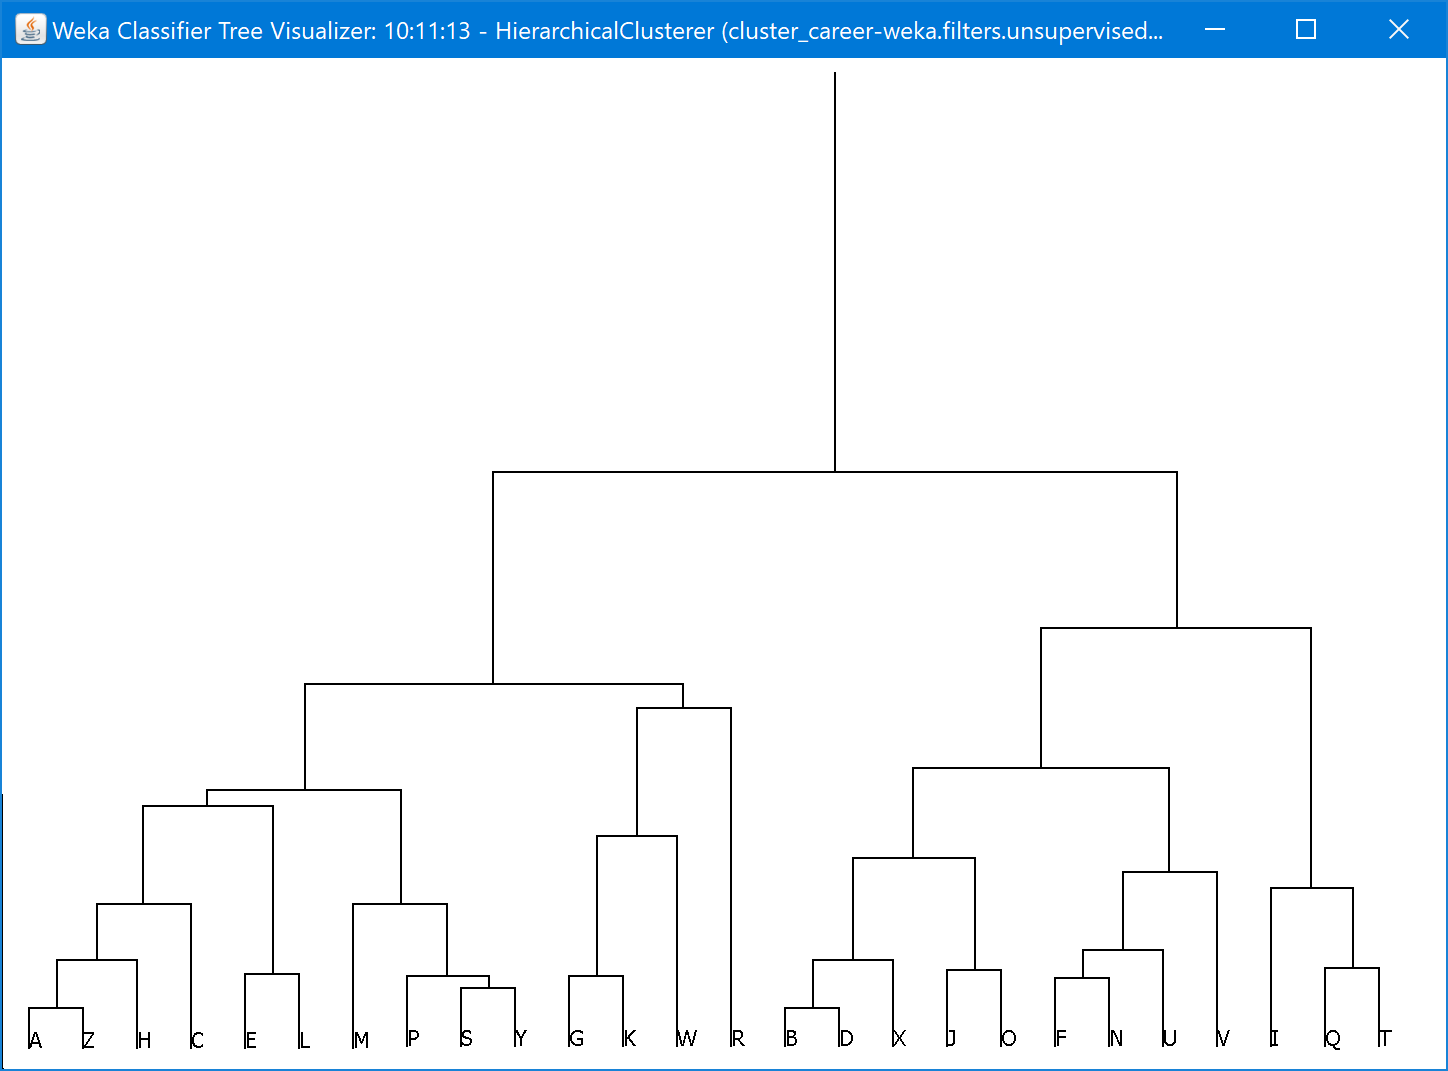
\includegraphics[scale=0.6]{Img/clustering_gerarchico_career_complete.png}
	\caption{Clustering gerarchico Complete Link su \textit{cluster\_career}.
		\label{fig:3}}
\end{figure} 

Inizialmente \`{e} stata fatta un'analisi per capire il numero di cluster nascosti nel dataset. Per questo scopo \`{e} stato utilizzato l'algoritmo di clustering gerarchico agglomerativo con metodo \textit{Complete Link}, al fine di usare opportunamente un metodo robusto per gestire gli \textit{outliers} presenti ed eventuale rumore nei dati. L'algoritmo \`{e} stato eseguito utilizzando come funzione di distanza quella Euclidea, selezionando un numero di cluster pari ad 1 (per non ricercare un numero di cluster specifico), lasciando tutti gli altri parametri di default e selezionando i primi tre attributi della vista (test\_grade, hs\_diploma\_grade, grade\_weighted\_avg), questo giustificato dal fatto che, come mostrato in precedenza, sono gli attributi pi\`{u} correlati tra loro e quindi pi\`{u} significativi.

Come si pu\`{o} vedere dal dendogramma risultante in Figura \ref{fig:3}, l'algoritmo divide il set in due principali cluster. Per avere una conferma di questo raggruppamento \`{e} stato utlizzato sul set anche il metodo \textit{Group Avarage} ottenendo il dendogramma in Figura \ref{fig:4}.

\begin{figure}[!]
	\centering
	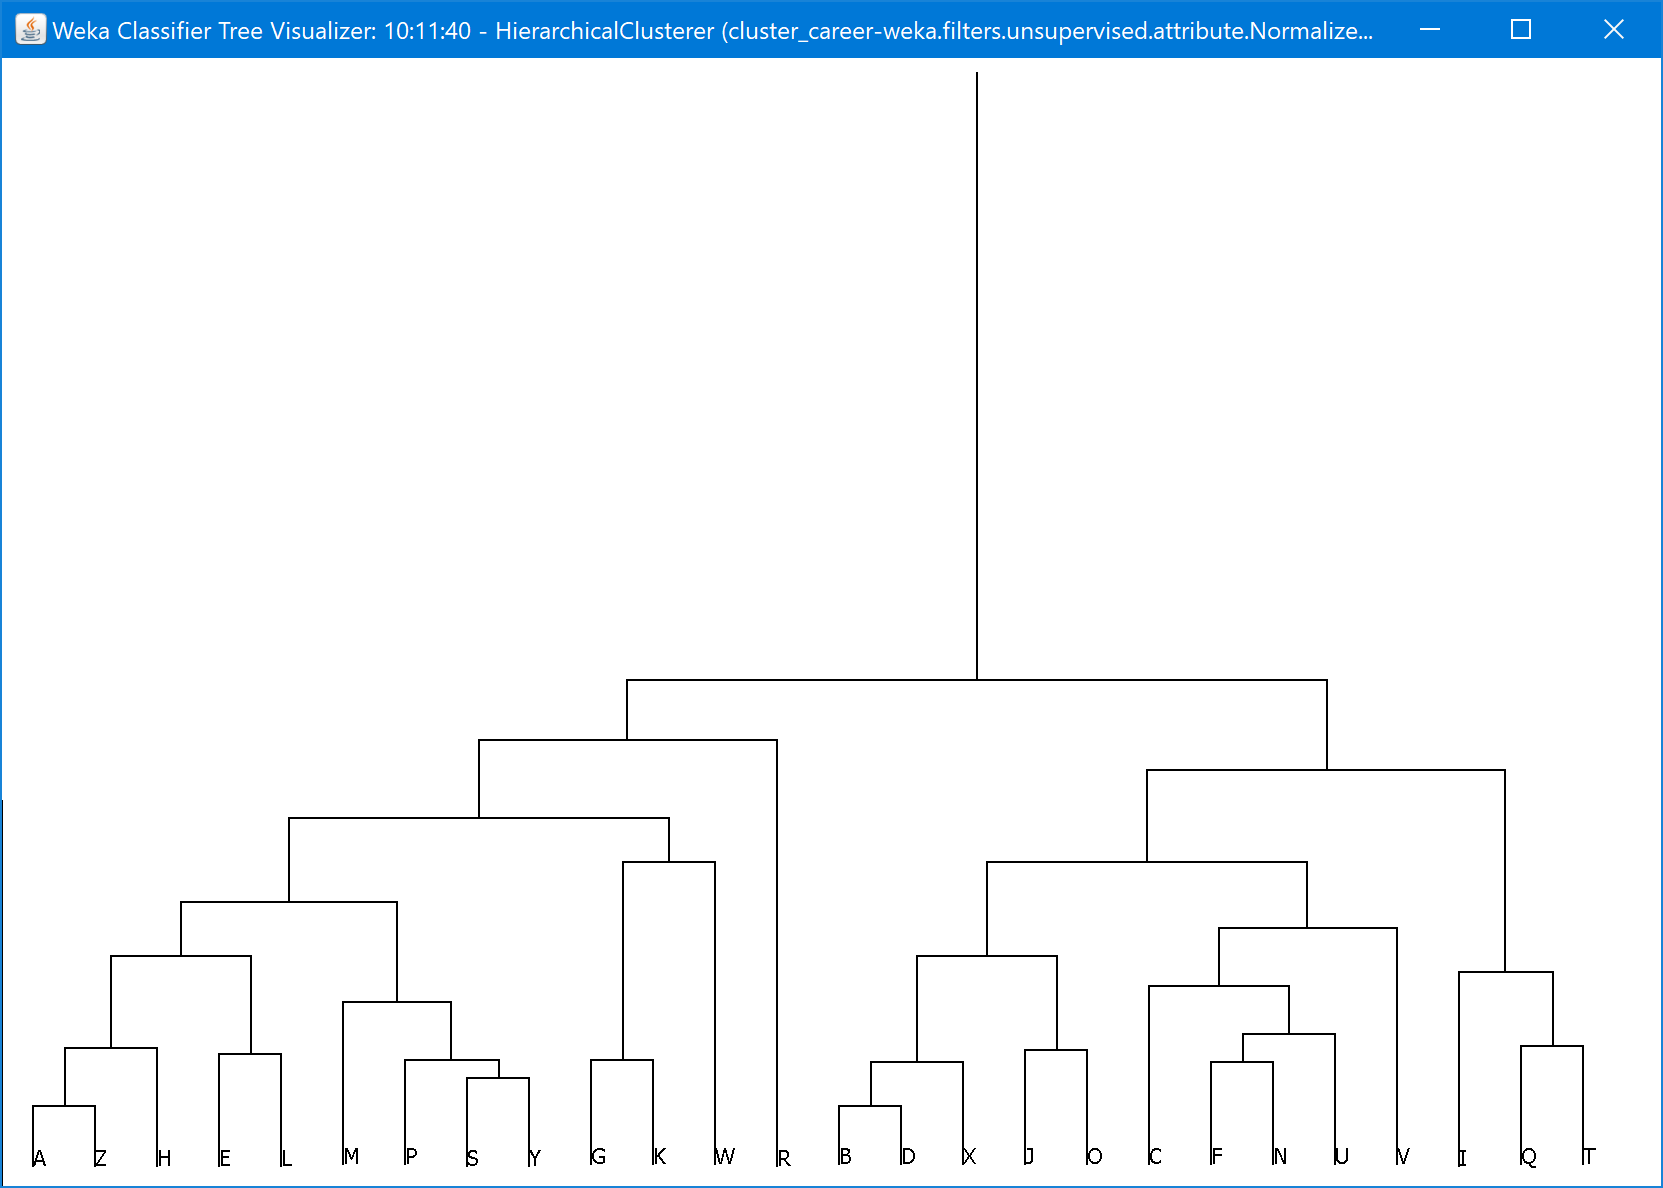
\includegraphics[scale=0.5]{Img/clustering_gerarchico__career_average.png}
	\caption{Clustering gerarchico Group Avarage su \textit{cluster\_career}.
		\label{fig:4}}
\end{figure} 

Anche in questo caso si \`{e} avuta la conferma che i cluster nascosti sono principalmente due. \\

Prima di eseguire un algoritmo di clustering ricercando un numero di cluster specifico sono state fatte alcune prove anche utilizzando l'algoritmo \textit{DB-Scan} non ottentendo per\`{o} risultati soddisfacenti dovuti probabilmente al fatto di operare con un database molto ridotto e poco denso.\\

Appurato quindi che i cluster principali sono due, l'insieme dei dati \`{e} stato analizzato usando l'algoritmo \textit{k-means} implementato in Weka, eseguito utilizzando la distanza Euclidea, specificando due cluster da ricercare e lasciando i valori di default per la generazione casuale dei centroidi (seed = 10).

L'algoritmo k-means \`{e} stato eseguito con due configurazioni di dati, la prima, come fatto per l'algoritmo di clustering gerarchico, considerando solo i primi tre attributi della vista (\textit{test\_grade},\textit{hs\_diploma\_grade}, \textit{grade\_weighted\_avg}) ed ignorando tutti gli altri. I risultati ottenuti sono, una proporzione del $50\%$ degli studenti assegnata ad ogni cluster (13 studenti in tutti e due i cluster su un totale di 26 studenti), un SSE pari a $3.19$ ed i seguenti centroidi.

\begin{center}
	\resizebox{\columnwidth}{!}{
		\begin{tabular}{llll}
			\hline
			Cluster & test\_grade & hs\_diploma\_grade & grade\_weighted\_avg \\ \hline
			0 & 0.5315 & 0.659 & 0.6044 \\
			1 & 0.4406 & 0.3056 & 0.0659 \\ \hline
		\end{tabular}
	}
\end{center}

In particolare nella Figura \ref{fig:5} viene mostrata l'assegnazione di ogni studente al suo cluster. Mentre nella Figura \ref{fig:6} viene mostrato il plot di incrocio tra i due attributi pi\`{u} correlati (\textit{hs\_diploma\_grade} e \textit{grade\_weighted\_avg}).

\begin{figure}[!]
	\centering
	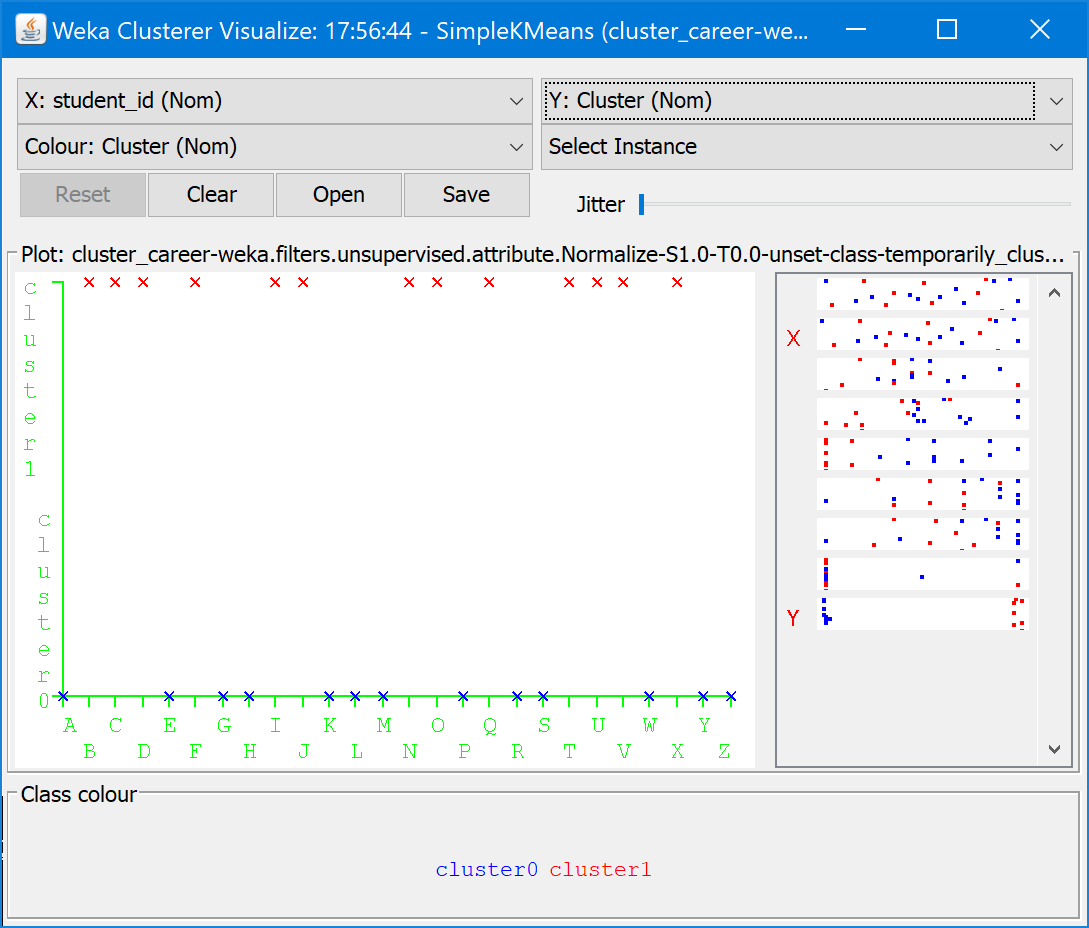
\includegraphics[scale=0.6]{Img/kmeans_career_3attributi_assegnamenti.png}
	\caption{Assegnazioni k-means clustering (3 attributi) su \textit{cluster\_career}.
		\label{fig:5}}
\end{figure} 

\begin{figure}[!]
	\centering
	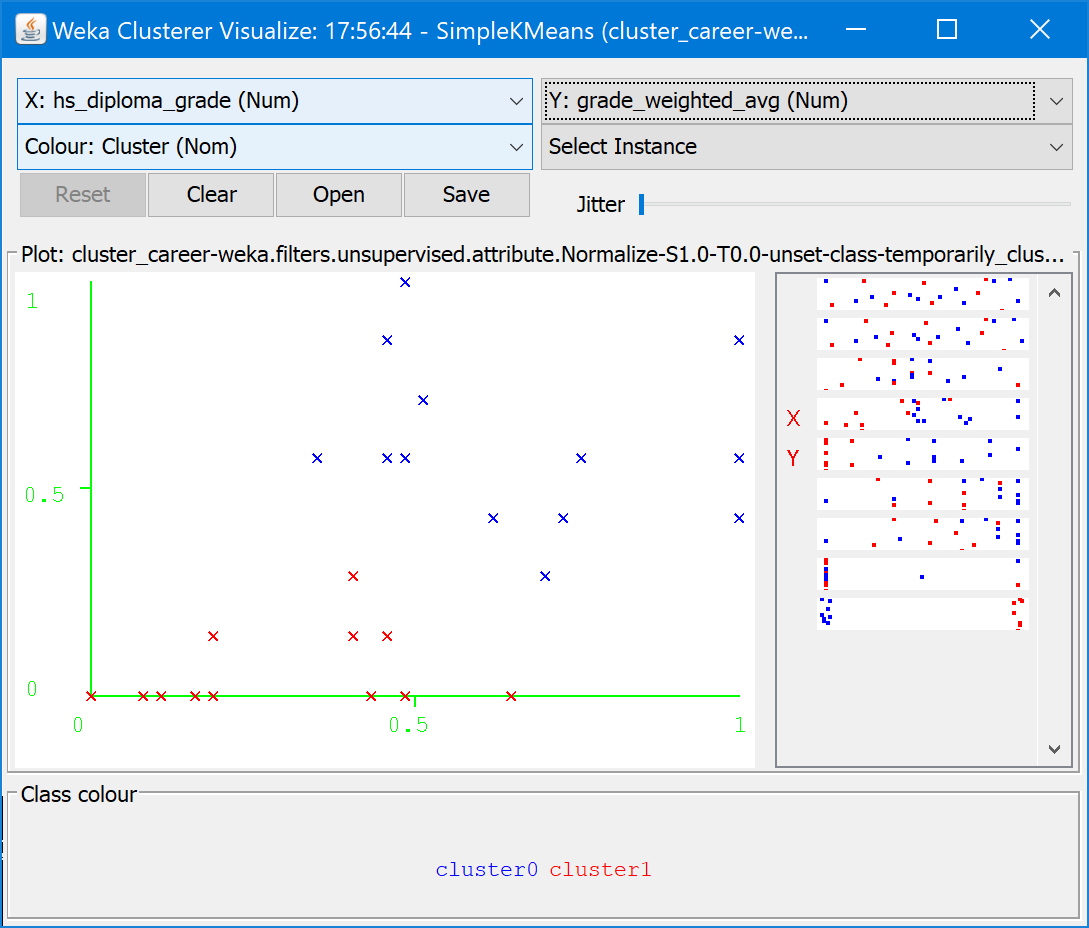
\includegraphics[scale=0.6]{Img/kmeans_career_3Attributi_incrocio.png}
	\caption{k-means clustering su \textit{cluster\_career} (3 attributi), incrocio fra due attributi.
		\label{fig:6}}
\end{figure} 

Successivamente, durante la seconda esecuzione del k-means, sono stati considerati tutti gli attributi della vista, escludendo solo lo \textit{student\_id}. I risultati ottenuti in questo caso sono, una proporzione del $46\%$ (12 studenti) assegnata al cluster 0 ed una proporzione del $54\%$ (14 studenti) assegnata al cluster 1, un SSE pari a $8.37$ ed i seguenti centroidi:

\begin{center}
	\resizebox{\columnwidth}{!}{
		\begin{tabular}{lllllll}
			\hline
			Cluster & test\_grade & hs\_diploma\_grade & grade\_weighted\_avg & exams\_taken & total\_cfu & years \\ \hline
			0 & 0.553 & 0.6486 & 0.5476 & 0.9167 & 0.914 & 0.125 \\
			1 & 0.4286 & 0.3398 & 0.1531 & 0.513 & 0.5115 & 0.1429 \\ \hline
		\end{tabular}
	}
\end{center}

Nella Figura \ref{fig:7} viene mostrata l'assegnazione di ogni studente al suo cluster. Mentre nella Figura \ref{fig:8} viene mostrato il plot di incrocio tra i due attributi pi\`{u} correlati.

\begin{figure}[!]
	\centering
	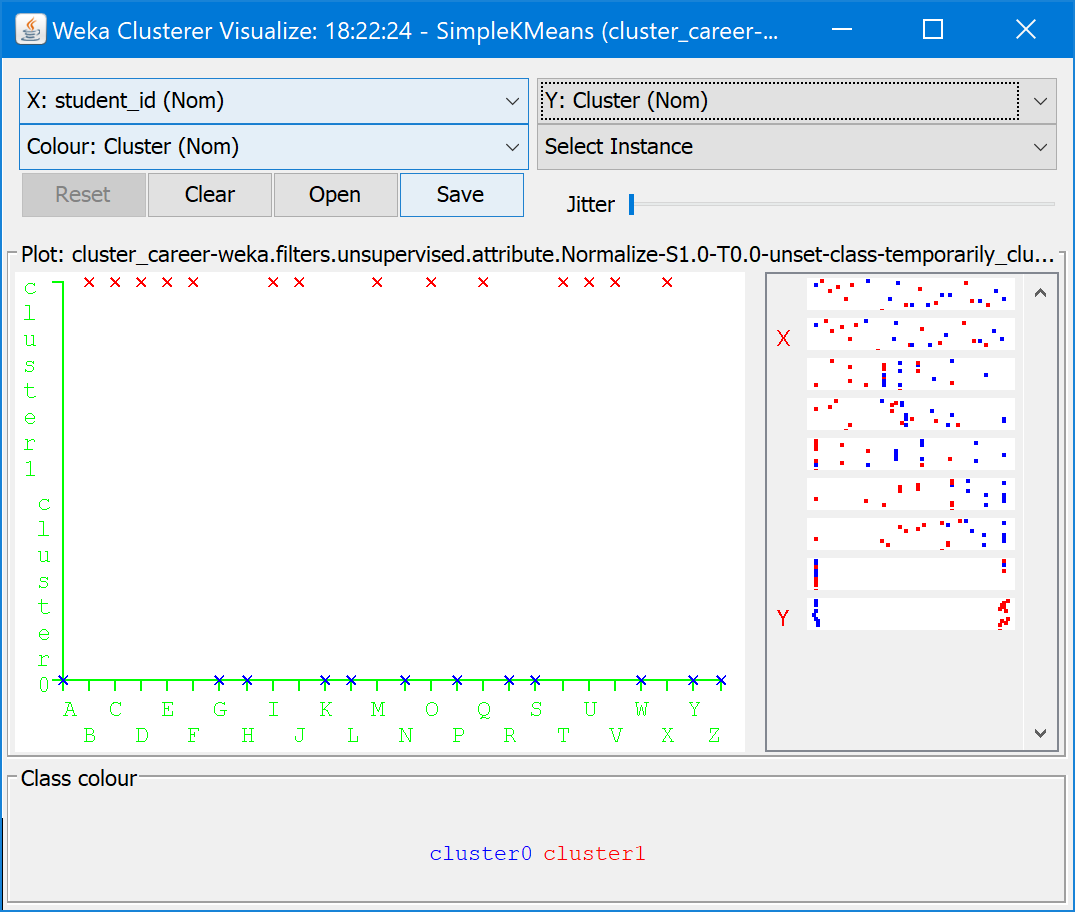
\includegraphics[scale=0.6]{Img/kmeans_career_allAttributi_assegnamenti.png}
	\caption{Assegnazioni k-means clustering su \textit{cluster\_career}.
		\label{fig:7}}
\end{figure} 

\begin{figure}[!]
	\centering
	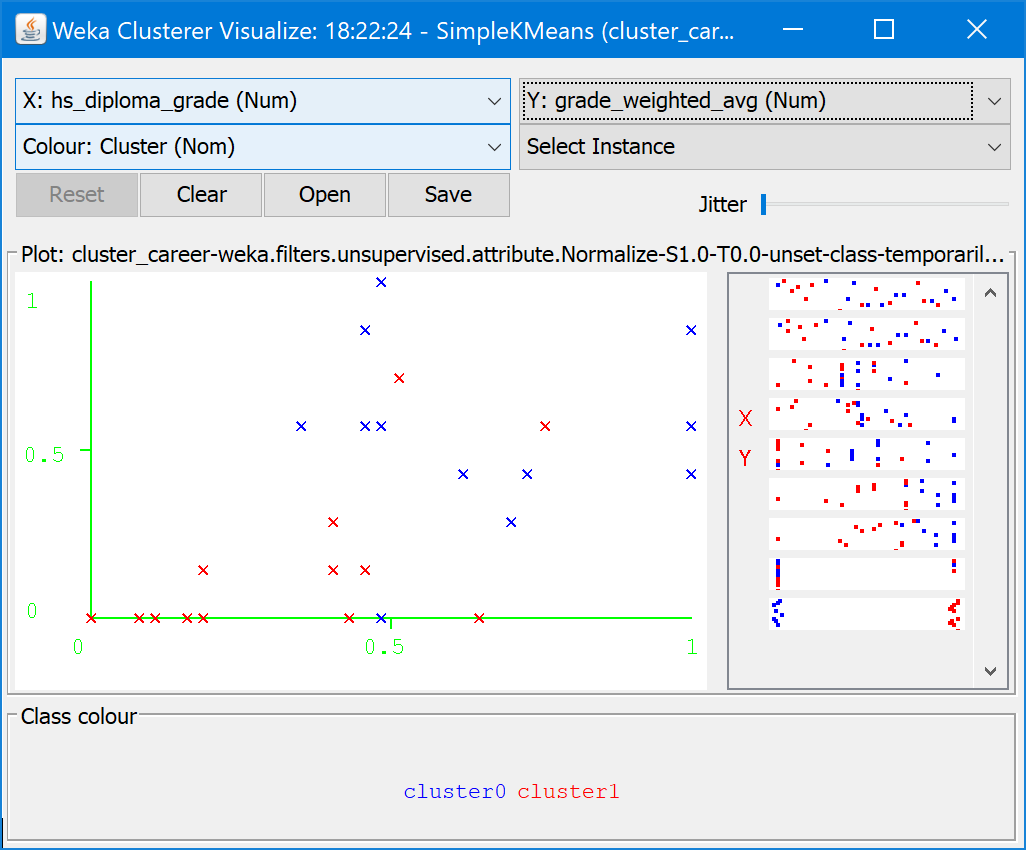
\includegraphics[scale=0.65]{Img/kmeans_career_allAttributi_incrocio.png}
	\caption{k-means clustering su \textit{cluster\_career}, incrocio fra due attributi.
		\label{fig:8}}
\end{figure} 

Analizzando i risultati dei centroidi e degli assegnamenti, si pu\`{o} notare come in entrambi i casi, gli studenti siano divisi in due categorie, in base alla loro appartenenza ad uno o all'altro cluster, quella degli studenti con un miglior percorso, ovvero quelli con una miglior carriera universitaria, e quella relativa agli studenti con un percorso peggiore, evidenziato anche dalla Figura \ref{fig:9}.\\ 
Come si pu\`{o} vedere nelle Figure \ref{fig:6} e \ref{fig:8}, i due gruppi sono chiaramente visibili e separati in base ai risultati ottenuti dagli studenti durante la loro carriera universitaria. La differenza principale tra le due sta in alcuni studenti che, pur avendo ottenuto voti abbastanza alti durante la loro carriera universitaria, hanno sostenuto pochi esami e che quindi vengono penalizzati nel seconda operazione di clustering, in quanto viene tenuto conto anche del numero e dell'importanza (cfu) degli esami dati. \\

\begin{figure}[!]
	\centering
	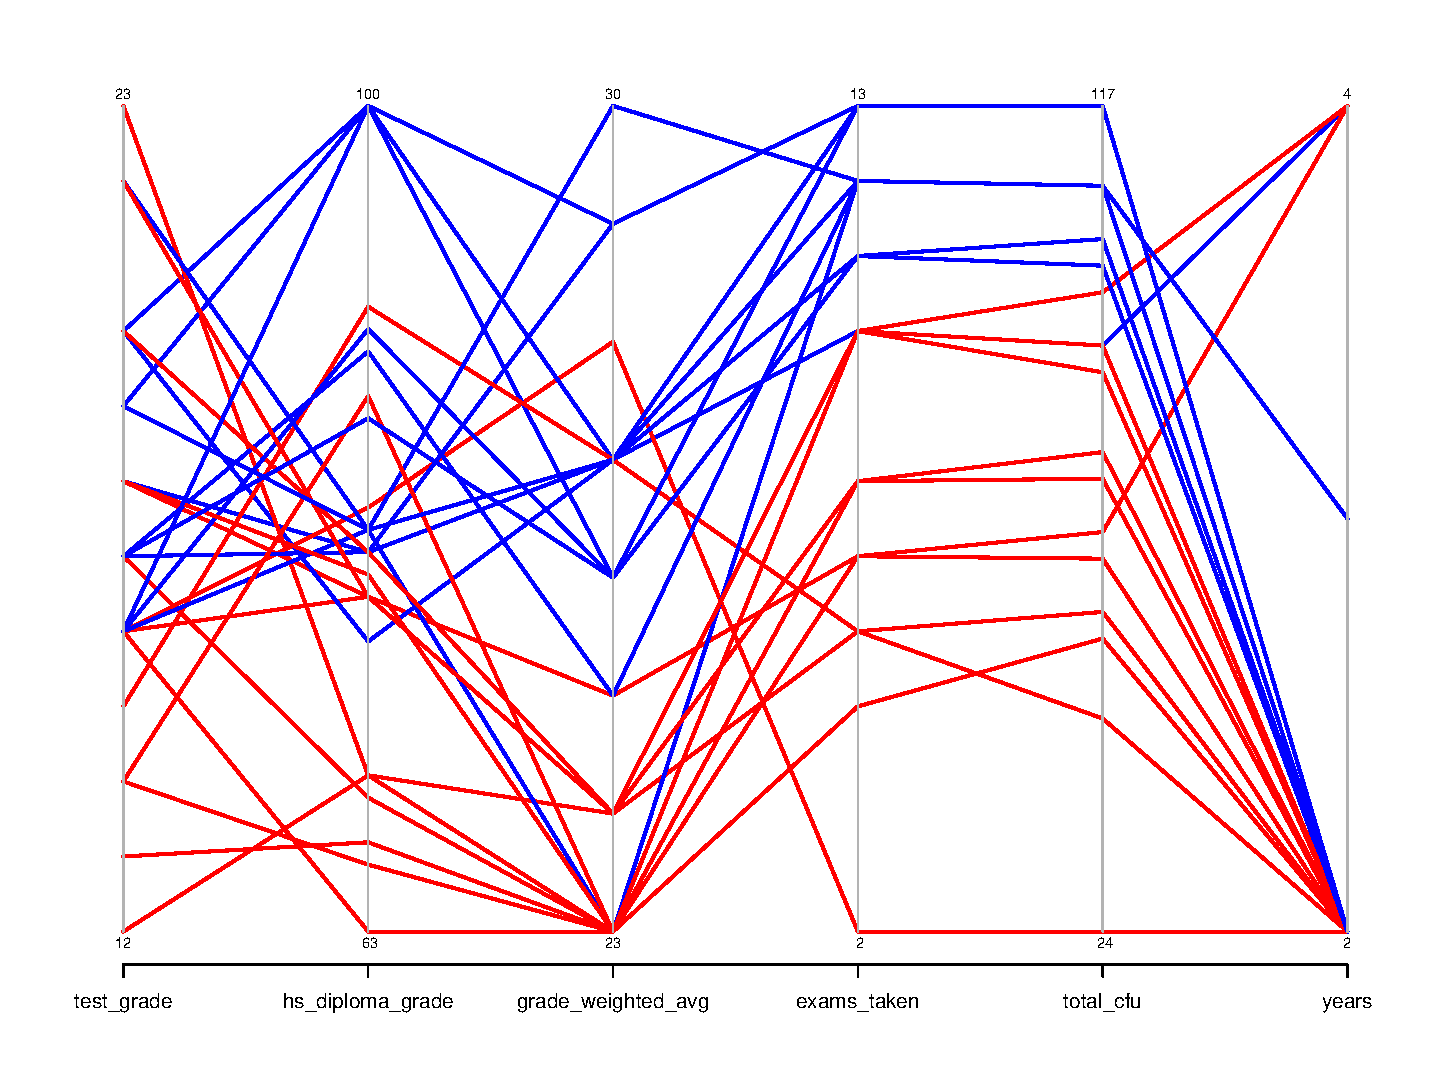
\includegraphics[scale=0.45]{Img/parallel_coord_career.pdf}
	\caption{Coordiante Parallele per il k-means clustering su \textit{cluster\_career}.
		\label{fig:9}}
\end{figure} 

Mostriamo ora le seconda analisi relativa all'andamento dei risultati di ogni esame degli studenti, usando i dati estrapolati dalla vista \textit{cluster\_exams}, aggiornando i dati mancanti come spiegato nella fase di preprocessing, e resi disponibili nel file \textit{cluster\_exams.csv}.\\

Anche in questo caso inizialmente \`{e} stata fatta un'analisi per capire il numero di cluster nascosti nel dataset utilizzando alcuni algoritmi di clustering gerarchici ed ottenendo come nel caso precedente un numero di lcuster nascosti pari a due. 

Appurato quindi che i cluster principali sono due, l'insieme dei dati \`{e} stato analizzato usando l'algoritmo \textit{k-means}, eseguito utilizzando la distanza Euclidea, specificando due cluster da ricercare e lasciando i valori di default per la generazione casuale dei centroidi (seed = 10). I risultati ottenuti sono, una proporzione del $50\%$ degli studenti assegnata ad ogni cluster (13 studenti in tutti e due i cluster su un totale di 26 studenti), un SSE pari a $17.96$ ed i seguenti centroidi.

\begin{center}
	\resizebox{\columnwidth}{!}{
		\begin{tabular}{llllllllllllll}
			\hline
			Cluster & B006800 & B006801 & B006802 & B006803 & B006804 & B006807 & B006808 & B006813 & B006818 & B015325 & B018756 & B018757 & B018760 \\ \hline
			0 & 29.2308 & 28.3077 & 26.2436 & 25.7324 & 27.8846 & 27.859 & 23.3462 & 27.8077 & 26.0821 & 25.6875 & 28.0734 & 28.1667 & 28.1247 \\
			1 & 24.5385 & 24.1165 & 21.1282 & 22.5961 & 25.1667 & 22.578 & 23.7415 & 22.7584 & 23.0661 & 23.6839 & 25.0238 & 23.9648 & 22.028 \\ \hline
		\end{tabular}
	}
\end{center}

In particolare nella Figura \ref{fig:10} viene mostrata l'assegnazione di ogni studente al suo cluster. Mentre nella Figura \ref{fig:11} viene mostrato il plot di incrocio tra i due attributi pi\`{u} correlati (ASD e CPS).

\begin{figure}[!]
	\centering
	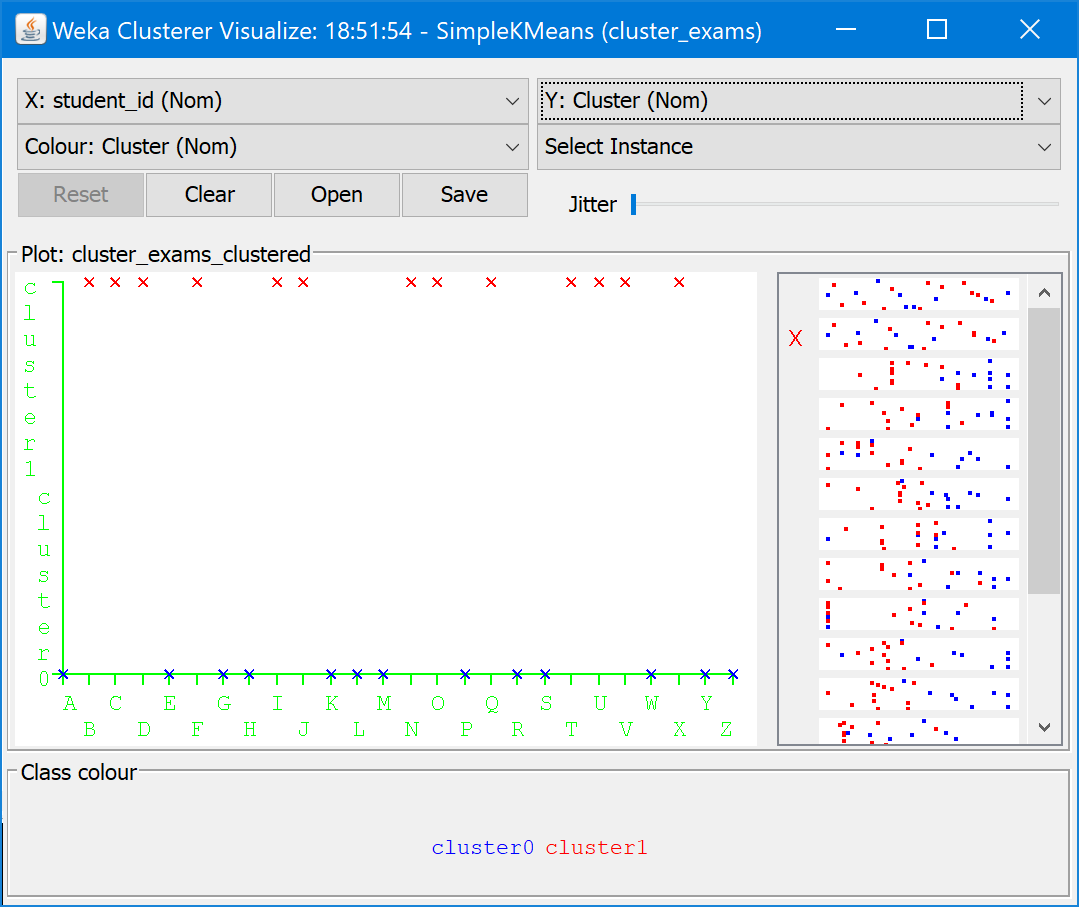
\includegraphics[scale=0.6]{Img/kmeans_exams_assegnamenti.png}
	\caption{Assegnazioni k-means clustering su \textit{cluster\_exams}.
		\label{fig:10}}
\end{figure} 

\begin{figure}[!]
	\centering
	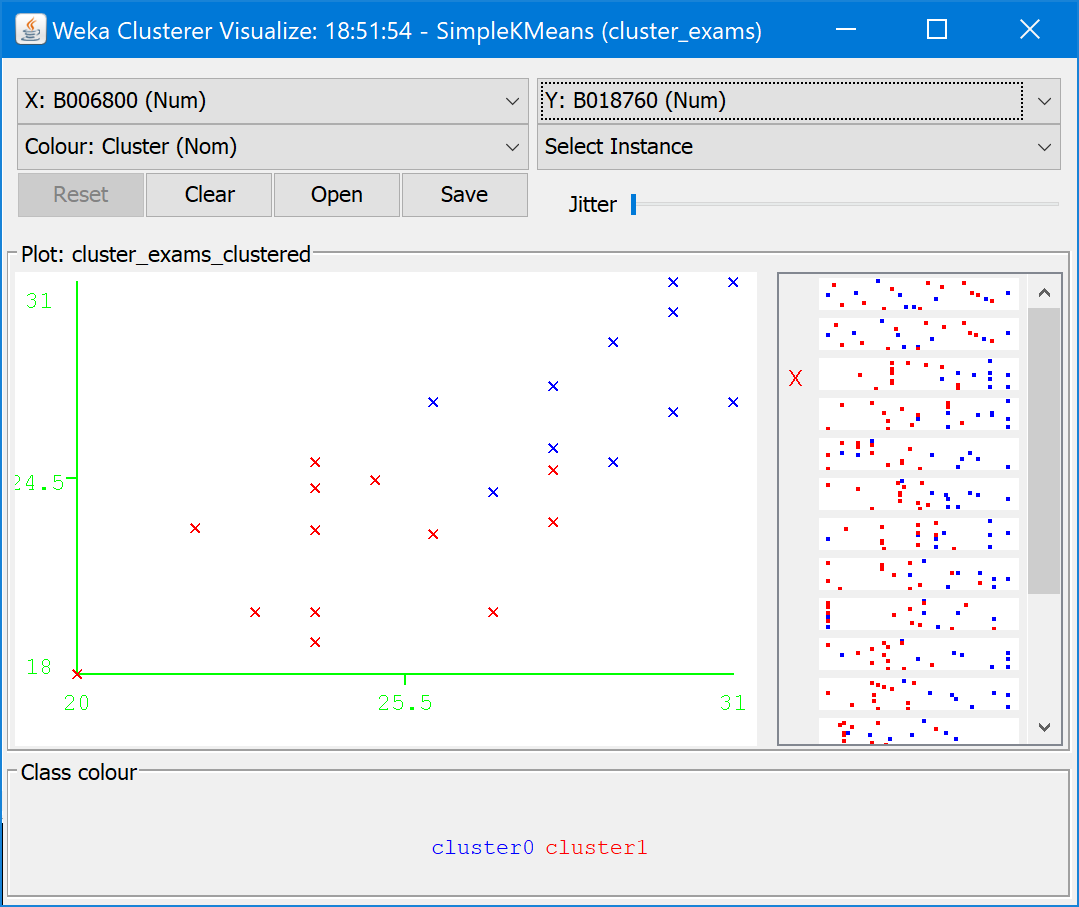
\includegraphics[scale=0.6]{Img/kmeans_exams_incrocio.png}
	\caption{k-means clustering su \textit{cluster\_exams}, incrocio fra ASD e CPS.
		\label{fig:11}}
\end{figure} 

Analizzando i risultati dei centroidi e degli assegnamenti, si pu\`{o} notare come anche in questo caso gli studenti siano divisi in due categorie, quella degli studenti con una sequenza di voti pi\`{u} alti e quella relativa agli studenti con una sequenza di voti peggiore. Inoltre si nota, osservando la Figura \ref{fig:10} come gli assegnamenti ai cluster siano molto simili (si differenziano per alcuni studenti assegnati diversamente) a quelli ottenuti per il clustering sulla carriera degli studenti confermando dunque l'accuratezza del clustering precedente come raggruppamento delle carriere ottimali e di quelle meno positive. Guardando la Figure \ref{fig:11} possiamo vedere come sono stati formati i due gruppi, chiarimenti visibili, se confrontati su i due attributi pi\`{u} correlati.

\section{Postprocessing e Classificazione}

Come ultima analisi si \`{e} voluto cercare di assegnare una particolare classe agli studenti per poi applicare al dataset un algoritmo di classificazione per comprendere se ci sia un modo, attraverso il dataset fornito, di prevedere se la carriera e il percorso intrapreso da uno studente sia "positivo" o "negativo", ovvero se lo studente riuscir\`{a} ad ottenere una carriera soddisfacente o meno, basando tale previsione sugli attributi gi\`{a} visti per la vista \textit{cluster\_career}

Per eseguire quest'ultima analisi per il \textit{training set} si \`{e} deciso di scegliere le classi basandoci sulle assegnazioni ai cluster ottenute per i risultati del clustering sulla carriera, ovvero, sulle assegnazioni mostrate in Figura \ref{fig:8} sulla vista \textit{cluster\_career}.

Una volta ottenuto le assegnazioni attraverso il software Weka \`{e} stato creato il file \textit{classification\_career.csv} a partire dal file \textit{cluster\_career.csv} inserendo una nuova colonna "\textit{class}" dedicata appunto alle assegnazioni ottenute dai risultati del clustering sulla vista \textit{cluster\_career}, ottenendo una tabella simile a quella seguente (ne viene riportata solo una porzione).

\begin{center}
	\resizebox{\columnwidth}{!}{
		\begin{tabular}{llllllll}
			\hline
			student\_id & test\_grade & hs\_diploma\_grade & grade\_weighted\_avg & exams\_taken & total\_cfu & years & class \\ \hline
			A & 18 & 80 & 27.0 & 10 & 90 & 4 & positive \\
			B & 13 & 67 & 23.0 & 10 & 96 & 4 & negative \\
			C & 18 & 78 & 25.0 & 7 & 69 & 4 & negative \\
			D & 14 & 66 & 23.0 & 7 & 66 & 2 & negative \\
			E & 16 & 82 & 28.0 & 2 & 24 & 2 & negative \\ \hline
		\end{tabular}
	}
\end{center}

Ad ogni studente \`{e} stata assegnata la classe "\textit{positive}" nel caso in cui lo studente sia stato precedentemente assegnato al cluster 0 ottenuto nella fase di clustering oppure la classe "\textit{negative}" nel caso in cui lo studente sia stato precedentemente assegnato al cluster 1, in modo tale da rispettare i diversi raggruppamenti basati sulla qualit\`{a} della carriera e del percorso dello studente. In Figura \ref{fig:12} viene mostrato un grafico di riassunto sulle caratteristiche del training set \textit{classification\_career.csv} cos\`{i} creato.

\begin{figure}[t]
	\centering
	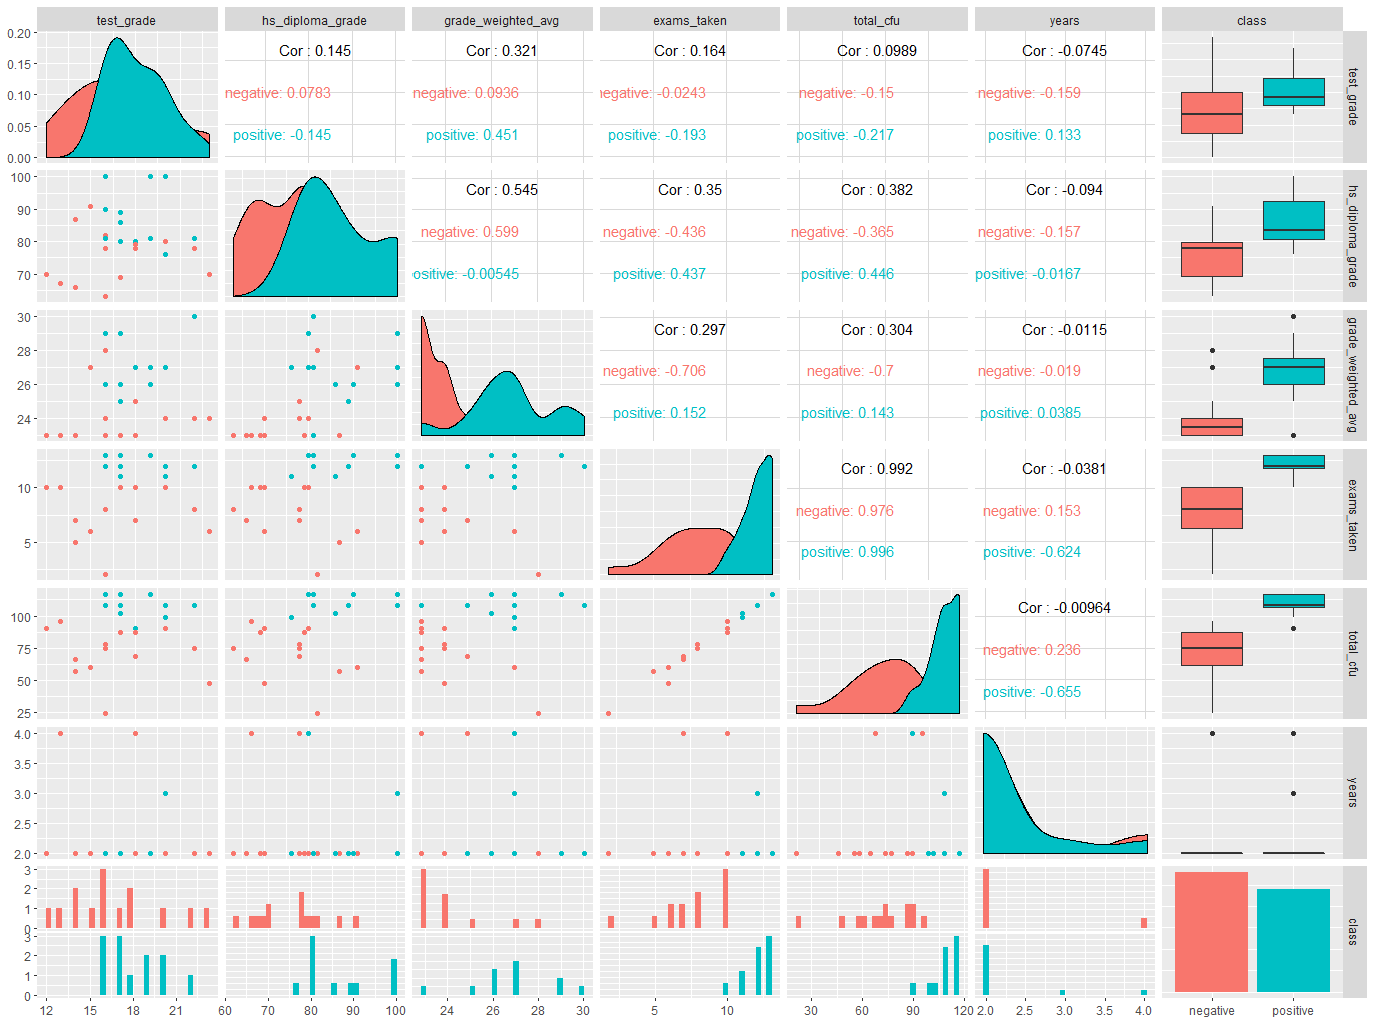
\includegraphics[scale=0.35]{Img/summary_class_plot.png}
	\caption{Grafico di riassunto del set \textit{classification\_career.csv}.
		\label{fig:12}}
\end{figure} 

A questo punto, il training set \textit{classification\_career.csv}, \`{e} stato importato in Weka e i vari attributi del set sono stati normalizzati direttamente attraverso tale software ad eccezione dello \textit{student\_id} e dell'attributo \textit{class}. Come algoritmo di classificazione \`{e} stato scelto il J48, per classificare tramite alberi di decisione, utilizzando i parametri di default, scegliendo come classe l'attributo \textit{class} del set e scegliendo come opzione per il test set il metodo \textit{Cross-Validation}.

I risultati ottenuti sono, una percentuale di istanze correttamente classificate pari al $96.15\%$ (\textit{Accuracy}) e una matrice di confusione riportata qui di seguito. Viene inoltre riportato in Figura \ref{fig:13} l'albero di decisione creato dall'algoritmo J48.

\begin{center}
	\resizebox{\columnwidth}{!}{
		\begin{tabular}{|c|c|c|c|}
			\hline
			& \multicolumn{3}{c|}{Predicted Class} \\ \hline
			\multirow{3}{*}{\begin{tabular}[c]{@{}c@{}}Actual\\  Class\end{tabular}} &  & Class=Positive & Class=Negative \\ \cline{2-4} 
			& Class=Positive & 11 & 1 \\ \cline{2-4} 
			& Class=Negative & 0 & 14 \\ \hline
		\end{tabular}
	}
\end{center}

\begin{figure}[t]
	\centering
	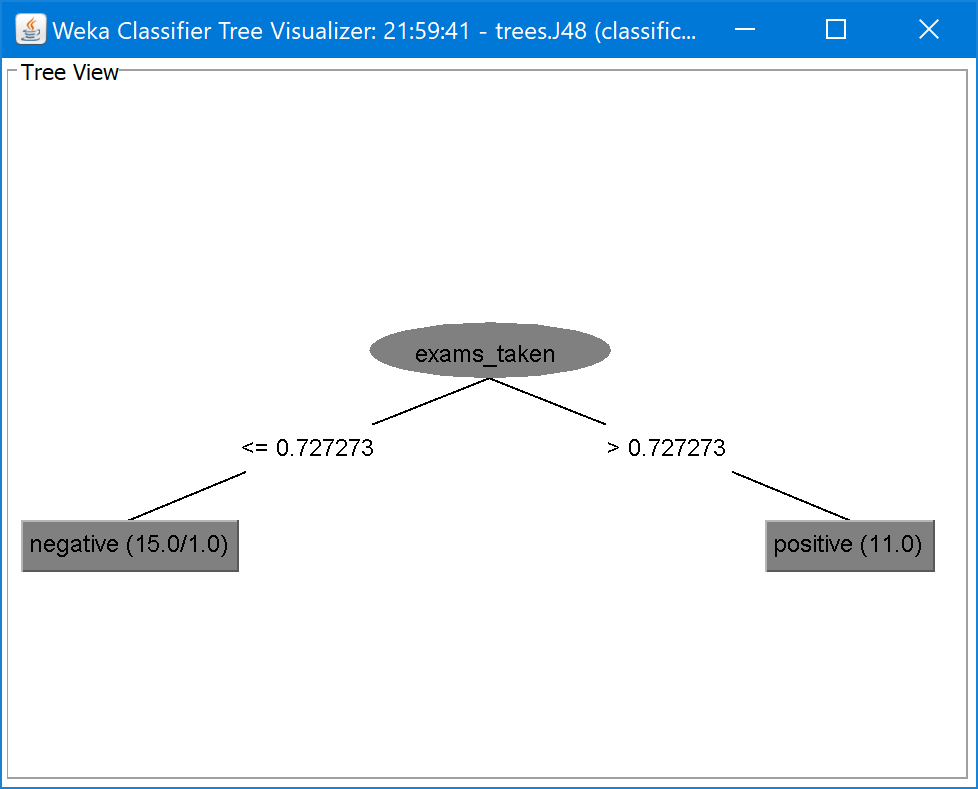
\includegraphics[scale=0.6]{Img/decision_tree.png}
	\caption{Albero di decisione.
		\label{fig:13}}
\end{figure} 

Purtroppo come \`{e} facilmente osservabile dalla Figura \ref{fig:13} i risultati della classificazione non sono molto interessanti dato che l'albero di decisione finale ha un solo livello e lo split scelto risulta essere un semplice controllo sul numero totale di esami dati, se quest'ultimi superano il valore normalizzato di circa $0.73$, che corrisponde ad un numero di esami pari a $10$ allora la carriera dello studente verr\`{a} classificata come "positiva" altrimenti sar\`{a} classificata come "negativa". Anche utilizzando altri tipi di metodi per la generazione del test set i risultati sono circa gli stessi, ottenendo quasi sempre una classificazione con un accuratezza del $96.15\%$ e dunque corrispondente ad un solo studente classificato in modo errato. 

I risultati ottenuti sulla classificazione sono per\`{o} sicuramente penalizzati dalla dimensione molto ridotta del dataset fornito e anche dal peso di molti datti mancanti, sopratutto relativi agli esami sostenuti.

\end{document}



